
\section{Simulação}

A distribuição de Poisson descreve contagem de eventos por unindade de tempo,
distância, área, volume, e mais. Sua função de massa de probabilidade é dada
por:

\begin{center}
  $P(X=x)=\dfrac{\lambda^{x}e^{-x}}{x!}, \quad E(X)=Var(X)=\lambda,$
\end{center}

\noindent onde $\lambda$ é a média da contagem por unidade de tempo, distância,
etc. Constam na figura \ref{Figure041-PoissonDistribution} distribuições de
Poisson para alguns valores de $\lambda$.

Para que uma variável aleatória siga a distribuição de Poisson, os eventos devem
ser independentes e a probabilidade de um evento ocorrer não pode variar com o
decorrer do tempo \cite{JBstatisticsPoissonIntroduction}
\cite{JBstatisticsPoissonOrNot}. Aplicada a este trabalho, a distribuição de
Poisson descreve a contagem de erros de trechos de código por execução.

Como o projeto de pesquisa se encontra em fase inicial, discussões e análises se
darão por meio de simulação. Um grafo mapa com $n$ vértices foi gerado e, com
probabilidade $p=0,5$, uma aresta de peso unitário pode ou não unir um par de
vértices quaisquer.

Para um valor arbitrário de $\lambda$, valores aleatórios da
distribuição de Poisson foram gerados para cada aresta do grafo mapa simulado.
Os valores em questão representam o número de falhas encontradas em uma execução
do software. O número de execuções simuladas foi de $1\mathrm{e}{+4}$ e o
parâmetro Poisson utilizado de $\lambda=5$.

{
  \centering
  \captionsetup{type=figure}
	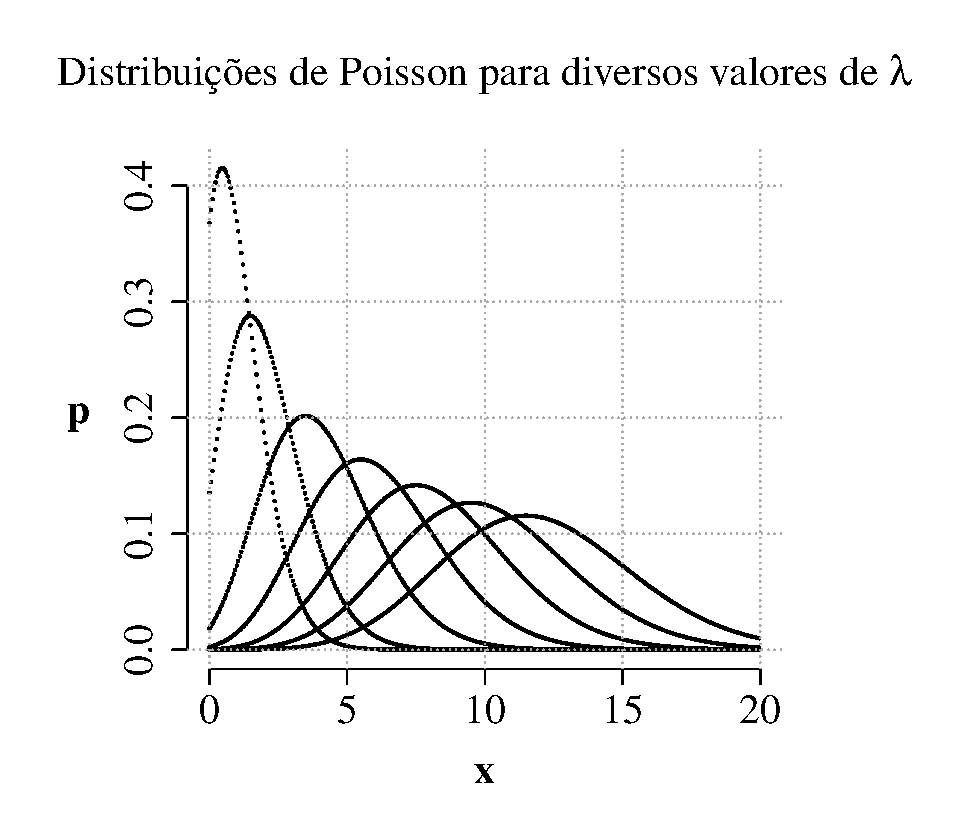
\includegraphics[scale=0.45]{./figures/Figure041-PoissonDistribution.pdf}
  \captionof{figure}{
    distribuições de Poisson para valores de $\lambda \in \{ 1, 2, 4, 6, ... \}$.
  }
	\label{Figure041-PoissonDistribution}
}
